\documentclass[11pt]{article}

\usepackage{graphicx}
\usepackage[top=25mm, bottom=25mm, left=25mm, right=25mm, a4paper]{geometry}
\usepackage{amsmath}
\usepackage{enumitem}
\usepackage{float}
\usepackage{fancyhdr}
\usepackage{booktabs}
\usepackage{upquote}
\usepackage{tikz}
\usepackage{steinmetz}

\pagestyle{fancy}
\fancyhf{}
\fancyhead[R]{Baturay Kafkas - 2240357068 - Electrical \& Electronics Engineering}

\rfoot{\thepage}
\renewcommand{\headrulewidth}{0pt} 
\renewcommand{\footrulewidth}{0pt}
\sloppy

\begin{document}

\begin{center}
\large
\textbf{ELE228 - Programming for Circuits and Systems Preliminary Work 5}
\end{center}

\section{Questions}

\begin{enumerate}[leftmargin=*,label=\textbf{\arabic*.}]
\item
    
\begin{enumerate}[leftmargin=*,label=\textbf{\theenumi\arabic*.}]
    \item Consider the circuit in \textit{Fig. 1}. Derive the numerical expression of the transfer function $H(s)=\frac{V_\text{out}(s)}{V_\text{in}(s)}$ for $R_1=100$ k$\Omega$ and $R_1=10$ k$\Omega$. Then find $H(j\omega)$ and cut--off frequencies ($f_c$). Comment on the filtering characteristics of the input--output relationship.
    \item Using MATLAB, write a code that finds the cut-off frequencies ($f_c$) from $H(s)$.
    \item Using MATLAB, plot the Bode diagram of systems in logarithmic scale (for $2$ different $R_1$ values in the same graph. Show cut-off frequencies in terms of Hz in the graph.
\end{enumerate}

\begin{figure}[h]
    \centering
    
\includegraphics[width=0.3\linewidth]{fig1.png}
    
    \textit{Figure 1}
\end{figure}

\item
    
\begin{enumerate}[leftmargin=*,label=\textbf{\theenumi\arabic*.}]
    \item Consider the circuit in \textit{Fig. 2}. Derive the numerical expression of the transfer function $H(s)=\frac{V_\text{out}(s)}{V_\text{in}(s)}$ for $R_1=100$ $\Omega$ and $R_1=1$ k$\Omega$. Then find $H(j\omega)$ and cut--off frequencies ($f_c$). Comment on the filtering characteristics of the input--output relationship.
    \item Using MATLAB, write a code that finds the cut-off frequencies ($f_c$) from $H(s)$.
    \item Using MATLAB, plot the Bode diagram of systems in logarithmic scale (for $2$ different $R_1$ values in the same graph. Show cut-off frequencies in terms of Hz in the graph.
\end{enumerate}

\begin{figure}[h]
    \centering
    
\includegraphics[width=0.3\linewidth]{fig2.png}

    \textit{Figure 2}
\end{figure}

\item
    
\begin{enumerate}[leftmargin=*,label=\textbf{\theenumi\arabic*.}]
    \item Consider the circuit in \textit{Fig. 3}. Derive the numerical expression of the transfer function $H(s)=\frac{V_\text{out}(s)}{V_\text{in}(s)}$ for $R_1=R_2=10$ k$\Omega$ and $R_3=R_4=100$ $\Omega$. Then find $H(j\omega)$ and cut--off frequencies ($f_c$) and bandwidth. Comment on the filtering characteristics of the input--output relationship.
    \item Using MATLAB, write a code that finds the cut-off frequencies ($f_c$) from $H(s)$.
    \item Using MATLAB, plot the Bode diagram of systems for linear scale and logarithmic scale (for 2 different resistance values in the same graph). Show cut-off frequencies in terms of Hz in the graph. Compare linear and logarithmic scales and explain why we use the logarithmic scale in Bode. Explain the advantages and disadvantages of higher-order filters.
\end{enumerate}

\begin{figure}[h]
    \centering
    
\includegraphics[width=0.55\linewidth]{fig3.png}

    \textit{Figure 3}
\end{figure}

\end{enumerate}

\newpage

\section{Answers}

\begin{enumerate}[leftmargin=*,label=\textbf{\arabic*.}]
\item
    
\begin{enumerate}[leftmargin=*,label=\textbf{\theenumi\arabic*.}]
    \item Impedance of the capacitor in the $s$--domain: $\frac1{sC}=\frac{10^7}{s}$. By the voltage divider,
    \[V_\text{out}=V_\text{in}\cdot\frac{R_1}{R_1+\frac{10^7}{s}},\quad \omega_c=\frac1{RC},\:f_c=\frac\omega{2\pi}\]
    \[R_1 = 100~\text{k}\Omega \implies H(s) = \frac{s}{s + 100},\:H(j\omega)=\frac{j\omega}{j\omega+100},\: w_c=100~\frac{\text{rad}}{\text{s}},\: f_c\approx 15.92~\text{Hz}\]
    \[R_1 = 10~\text{k}\Omega \implies H(s) = \frac{s}{s + 1000},H(j\omega)=\frac{j\omega}{j\omega+1000}, w_c=1000~\frac{\text{rad}}{\text{s}}, f_c\approx 159.2~\text{Hz}\]

    Both are high-pass filters. As the resistance increases, the circuit passes the input voltage to the output voltage starting from  lower frequencies. As the frequency of the input source decreases, the impedance of the capacitor increases. Therefore, the frequencies whose values are smaller than the cutoff value get attenuated.
    \item Code:
\vspace{1em}

\hrule
\begin{verbatim}
H_100k = tf([1, 0], [1, 100]);
H_10k = tf([1, 0], [1, 1000]);

p_100k = pole(H_100k);
fc_100k = abs(p_100k) / (2*pi)

p_10k = pole(H_10k);
fc_10k = abs(p_10k) / (2*pi)
\end{verbatim}
\hrule

\begin{figure}[H]
    \centering
    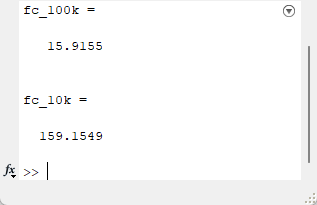
\includegraphics[width=0.45\linewidth]{MATLAB_GVrciFZ7Vm.png}

    \textit{Figure 4}
\end{figure}

\vspace{-1em}

\item Code:
\vspace{1em}

\hrule
\begin{verbatim}
bode_opt = bodeoptions;
bode_opt.Grid = 'on';
bode_opt.FreqScale = 'log';
bode_opt.FreqUnits = 'Hz';
bode_opt.Title.String = 'Bode Plot of H(s)';
bode_opt.Title.FontWeight = 'bold';
bode_opt.Title.FontSize = 12;

figure;
bodeplot(H_100k, H_10k, bode_opt);

axes = findall(gcf,'type','axes');
for k = 1:length(axes)
  xline(axes(k),fc_100k,'--k', sprintf('f_{c,100k} = %.2f Hz',fc_100k));
  xline(axes(k),fc_10k,'--k', sprintf('f_{c,10k} = %.2f Hz',fc_10k));
end
legend('R_1 = 100 k\Omega','R_1 = 10 k\Omega','location','southwest');
\end{verbatim}
\hrule

\vspace{-1em}
\begin{figure}[H]
    \centering
    
\includegraphics[width=0.65\linewidth]{fig5.png}
    
    \vspace{-0.6em}
    \textit{Figure 5}
\end{figure}

\end{enumerate}

\vspace{-1.5em}
\item

\begin{enumerate}[leftmargin=*,label=\textbf{\theenumi\arabic*.}]
    \item Impedance of the capacitor in the $s$--domain: $\frac1{sC}=\frac{10^7}{s}$. By the voltage divider,
    \[V_\text{out}=V_\text{in}\cdot\frac{\frac{10^7}{s}}{R_1+\frac{10^7}{s}},\quad \omega_c=\frac1{RC},\:f_c=\frac\omega{2\pi}\]
    \[R_1 = 100~\Omega \implies H(s) = \frac{10^5}{s + 10^5},\:H(j\omega)=\frac{10^5}{j\omega+10^5},\: w_c=10^5~\text{rad/s},\: f_c\approx 15915~\text{Hz}\]
    \[R_1 = 1~\text{k}\Omega \implies H(s) = \frac{s}{s + 10^4},\:H(j\omega)=\frac{10^4}{j\omega+10^4},\: w_c=10^4~\text{rad/s},\: f_c\approx 1591.5~\text{Hz}\]

    Both are low-pass filters. As the resistance increases, the circuit passes the input voltage to the resistor voltage starting from lower frequencies. As the frequency of the input source increases, the impedance of the capacitor decreases. Therefore, the frequencies whose values are greater than the cutoff value get attenuated.
    \item Code:
\vspace{1em}

\hrule
\begin{verbatim}
H_100 = tf([0, 10^5], [1, 10^5]);
H_1000 = tf([0, 10^4], [1, 10^4]);

p_100 = pole(H_100);
fc_100 = abs(p_100) / (2*pi)

p_1000 = pole(H_1000);
fc_1000 = abs(p_1000) / (2*pi)
\end{verbatim}
\hrule

\begin{figure}[H]
    \centering
    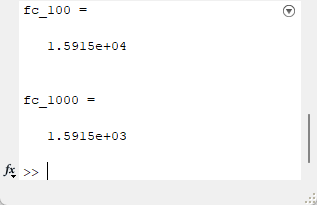
\includegraphics[width=0.45\linewidth]{MATLAB_TukseG74qW.png}

    \textit{Figure 6}
\end{figure}

\vspace{-1em}

\item Code:
\vspace{1em}

\hrule
\begin{verbatim}
bode_opt = bodeoptions;
bode_opt.Grid = 'on';
bode_opt.FreqScale = 'log';
bode_opt.FreqUnits = 'Hz';
bode_opt.Title.String = 'Bode Plot of H(s)';
bode_opt.Title.FontWeight = 'bold';
bode_opt.Title.FontSize = 11;

figure;
bodeplot(H_100, H_1000, bode_opt);

axes = findall(gcf,'type','axes');
for k = 1:length(axes)
  xline(axes(k),fc_100,'--k',sprintf('f_{c,100} = %.2f Hz',fc_100));
  xline(axes(k),fc_1000,'--k',sprintf('f_{c,1000} = %.2f Hz',fc_1000));
end

legend('R_1 = 100 \Omega','R_1 = 1000 \Omega','location','southwest');
\end{verbatim}
\hrule

\vspace{-1em}
\begin{figure}[H]
    \centering
    
\includegraphics[width=0.65\linewidth]{fig7.png}
    
    \vspace{-0.6em}
    \textit{Figure 7}
\end{figure}

\end{enumerate}

\newpage

\item
    
\begin{enumerate}[leftmargin=*,label=\textbf{\theenumi\arabic*.}]
\item Assign nodes.

\begin{figure}[H]
    \centering
    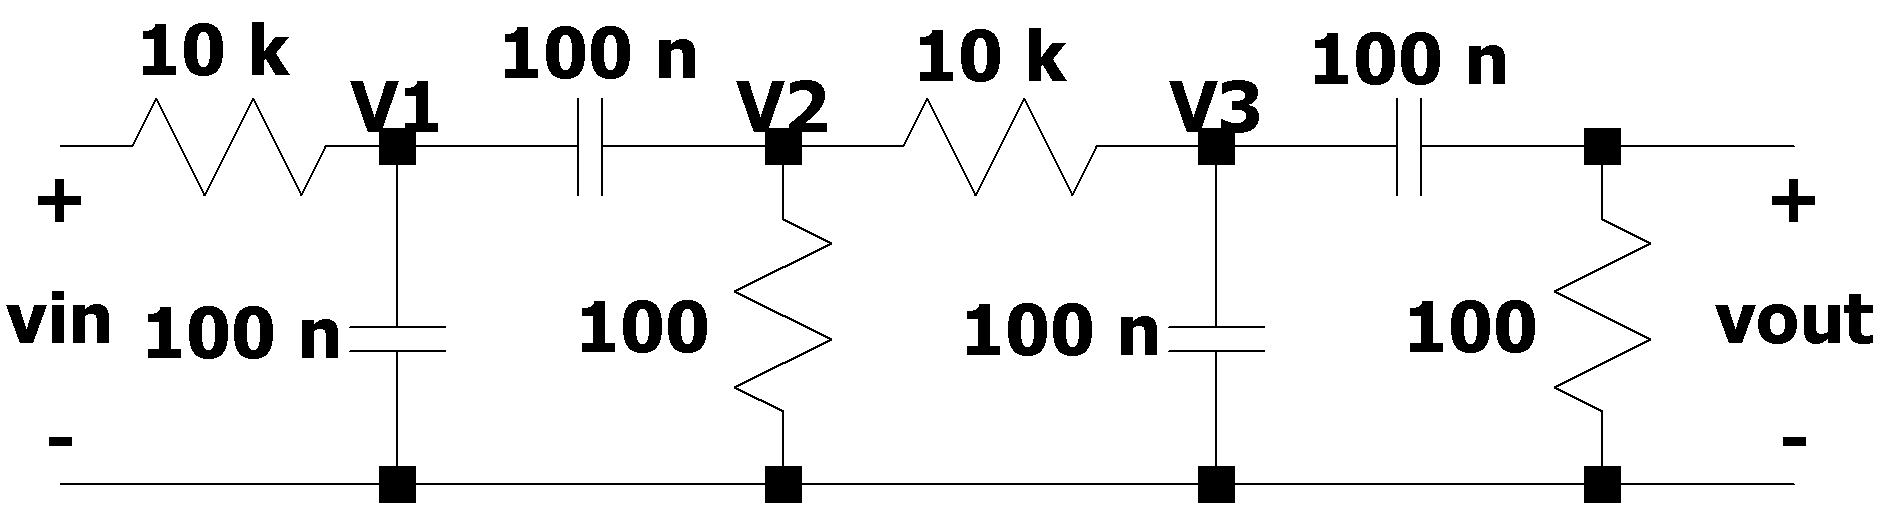
\includegraphics[width=0.65\linewidth]{fig8.png}
    
    \textit{Figure 8}
\end{figure}

Let the impedance of each capacitor be $Z_C$ in the $s$--domain. Apply KCL at each node.

\[\frac{V_1-V_\text{in}}{10~\text{k}}+\frac{V_1}{Z_C}+\frac{V_1-V_2}{Z_C}=0,\qquad\frac{V_2-V_1}{Z_C}+\frac{V_2}{100}+\frac{V_2-V_3}{10~\text{k}}=0,\]
\[\frac{V_3-V_2}{10~\text{k}}+\frac{V_3}{Z_C}+\frac{V_3-V_\text{out}}{Z_C}=0,\qquad\frac{V_\text{out}-V_3}{Z_C}+\frac{V_\text{out}}{100}=0.\]

$Z_C=\frac1{sC}=\frac1{s\cdot100\cdot10^{-9}}=\frac{10^7}s$. Equate and eliminate the denominators in each expression.
\[1000V_1+s(V_1+V_1-V_2)=1000V_\text{in},\quad s(V_2-V_1)+100000V_2+1000V_2-1000V_3=0\]
\[1000V_3-1000V_2+s(V_3+V_3-V_\text{out})=0,\quad s(V_\text{out}-V_3)+100000V_\text{out}=0.\]

%By the voltage divider,
%\[V_\text{out}=V_3\cdot\frac{10~\text{k}}{10~\text{k}+Z_C}=V_3\cdot\frac{s}{s+1000}.\]

Rearrange the equations and put in matrix form.

\[V_1(1000+2s)-V_2s=1000V_\text{in},\quad V_1(-s)+V_2(s+101000)-V_3\cdot1000=0\]
\[V_2(-1000)+V_3\left(1000+2s\right)-V_\text{out}s=0,\qquad V_3(-s)+V_\text{out}(s+100000)=0\]
\[\begin{bmatrix}
1000 + 2s & -s & 0 & 0 \\
-s & s + 101000 & -1000 & 0 \\
0 & -1000 & 1000 + 2s & -s \\
0 & 0 & -s & s + 100000
\end{bmatrix}
\begin{bmatrix}
V_1 \\
V_2 \\
V_3 \\
V_{\text{out}}
\end{bmatrix}
=
\begin{bmatrix}
1000V_{\text{in}} \\
0 \\
0 \\
0
\end{bmatrix}\]

Code:
\vspace{1em}

\hrule
\begin{verbatim}
syms s Vin
A = [1000+2*s, -s, 0, 0;
    -s, s+101000, -1000, 0;
    0, -1000, 1000+2*s, -s;
    0, 0, -s, s+100000];
B = [1000*Vin; 0; 0; 0];
V = A\B;
Vout = V(4);
H_sym = simplify(Vout / Vin);
[num_sym, den_sym] = numden(H_sym);
num_vec = double(coeffs(num_sym, s, 'All'));
den_vec = double(coeffs(den_sym, s, 'All'));
H = tf(num_vec, den_vec)
\end{verbatim}
\hrule

\begin{figure}[H]
    \centering
    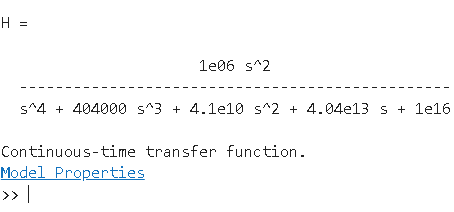
\includegraphics[width=0.5\linewidth]{chrome_tnN5N8O7Zz.png}    
    
    \textit{Figure 9}
\end{figure}

\[H(j\omega)=\frac{-10^6\omega^2}{\omega^4-404000j\omega^3-4.1\cdot10^{10}\omega^2+4.04\cdot10^{13}j\omega+10^{16}}\]

The poles are
\[p_1=-2.0292\cdot10^5,\quad p_2=-2.0009\cdot10^5,\quad p_3=-0.0050\cdot10^5,\quad p_4=-0.0049\cdot10^5.\]

The frequencies are then
\[f_1=3.2296\cdot10^4,\quad f_2=3.1845\cdot10^4,\quad f_3=0.0080\cdot10^4,\quad f_4=0.0078\cdot10^4\]

For the bandpass, $f_2$ and $f_3$ are meaningful. Therefore,
\[f_\text{c, lower}=80~\text{Hz},\quad f_\text{c, upper}=31845~\text{Hz}.\]

The bandwidth:
\[f_\text{c, upper}-f_\text{c, lower}=31845-80=31765~\text{Hz}\]

This circuit is a bandpass filter that passes the specific range of frequencies and attenuates the other frequencies.

\item Code:
\vspace{1em}

\hrule
\begin{verbatim}
p = pole(H); 
f_poles = abs(p) / (2*pi)
\end{verbatim}
\hrule

\begin{figure}[H]
    \centering
    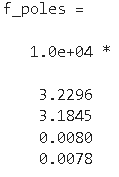
\includegraphics[width=0.15\linewidth]{chrome_Ye9AoJsaRy.png}

    \textit{Figure 10}
\end{figure}

Since this is a fourth-order bandpass filter, we take the frequencies that are closer to the band.
\[f_\text{cutoff, lower}=80~\text{Hz},\quad f_\text{cutoff, upper}= 31845~\text{Hz}\]

\newpage

\item Code:
\vspace{1em}

\hrule
\begin{verbatim}
scales = {'Log', 'Linear'};
figure;
for i = 1:2
    subplot(2, 1, i);
    bode_opt = bodeoptions;
    bode_opt.Grid = 'on';
    bode_opt.FreqScale = scales{i};
    bode_opt.FreqUnits = 'Hz';
    bode_opt.Title.String = ['Bode Plot (', scales{i}, ' Scale)'];
    bodeplot(H, bode_opt);
end

axes = findall(gcf,'type','axes');
for k = 1:length(axes)
    xline(axes(k),f_poles(3),'--k', ...
    sprintf('f_{c, upper} = %.2f Hz',f_poles(3)));
    xline(axes(k),f_poles(2),'--k', ...
    sprintf('f_{c, lower} = %.2f Hz',f_poles(2)));
end
\end{verbatim}
\hrule

\vspace{1em}

The plots are given in the next page.

\begin{figure}[H]
    \centering
    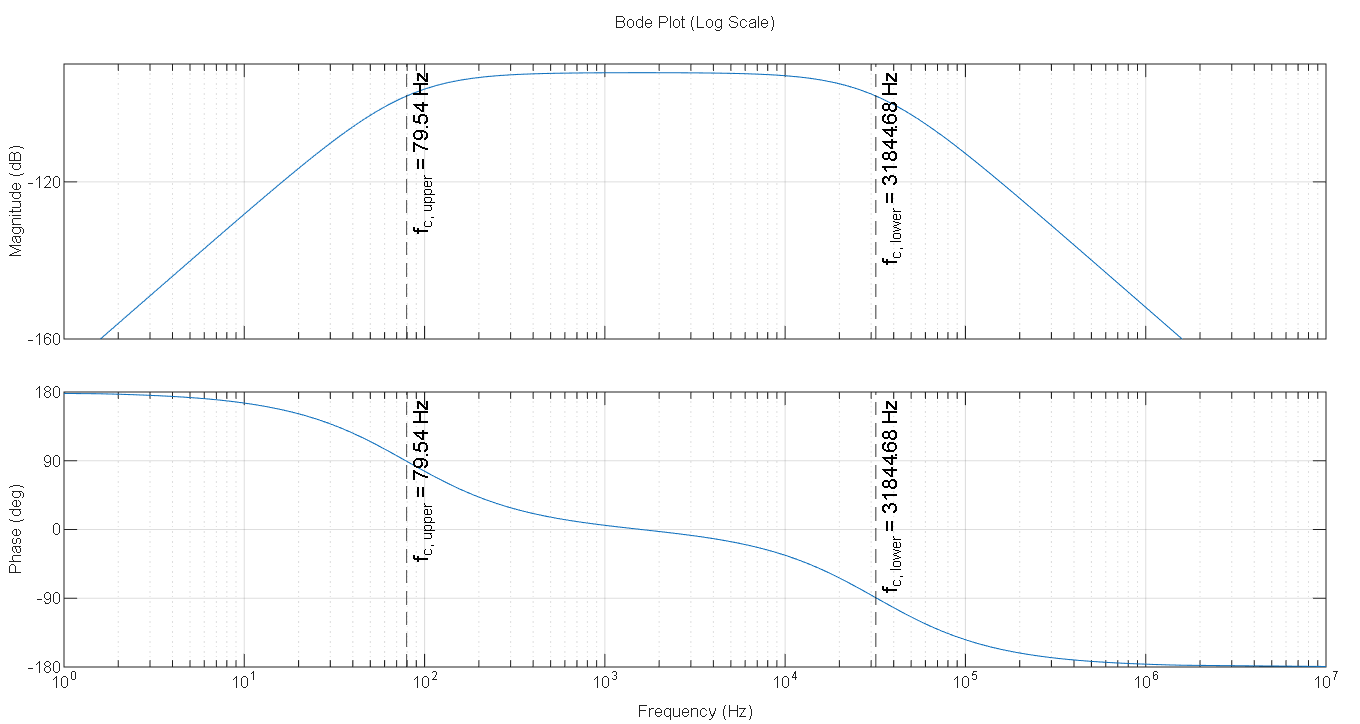
\includegraphics[width=1\linewidth]{exp5_3_1.png}    
    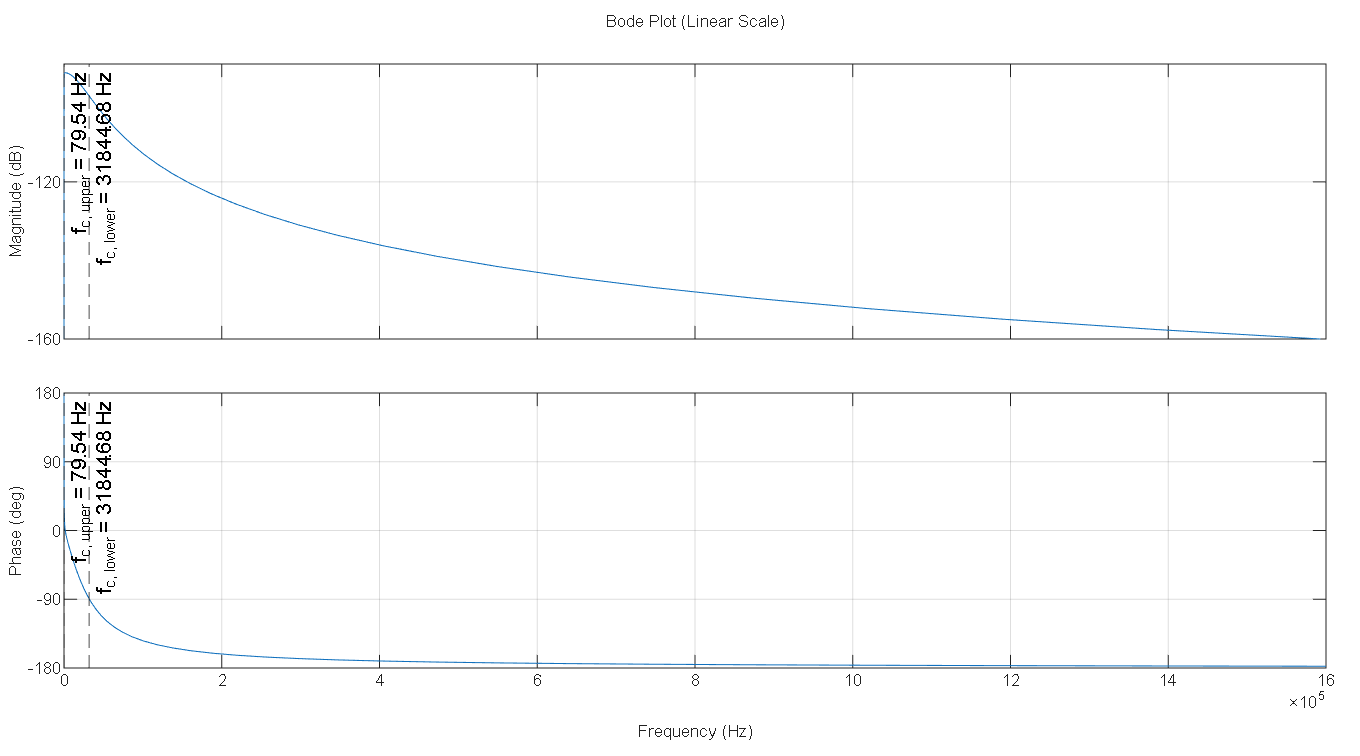
\includegraphics[width=1\linewidth]{exp5_3_2.png}    
    \textit{Figure 11}
\end{figure}

The main reason we use logarithmic scales in Bode plots is that they transform the complex exponential relationships of a circuit into straight lines, facilitating to visualize a filter's behavior across a range of frequencies. If we used the linear scale, we would struggle to analyze the cutoff frequencies as above.

The advantage of using high-order filters is that they select the certain frequency range that will be attenuated or passed, performing better compared to low-order ones. The disadvantage of using these filters is that the complexity of the circuit becomes higher, making calculations more difficult.

\end{enumerate}
\end{enumerate}

\end{document}